% !TEX root = ../Thesis.tex
%%
%%  Hochschule für Technik und Wirtschaft Berlin --  Abschlussarbeit
%%
%% Kapitel 3.5 - Vorarbeit
%%
%%

\chapter{Analyse der Air-Gap-Arbeitsumgebung und Tool-Chain} \label{Vorarbeit}



\section{Übersicht}
Vor Beginn der Bachelorarbeit wurde ein dreimonatiges Praktikum absolviert, was sich mit essentiellen Punkten zur Grundlagenbildung auseinander gesetzt hat. 

\subsection{Einführung in das Unternehmen}
Im Rahmen des Praktikums fand an erster Stelle eine Einführung in das Unternehmen selbst statt. So wurden Einblicke in die Organisationsstruktur und einzelne Abteilungen sowie Standorte gegen. Hierzu zählen unter anderem die technische Zentrale am Werner-Voß-Damm, wo der Großteil der Zeit verbracht wurde. Hier fand auch der Einblick in das operative Geschäft in Form von wöchentlichen Teamleitertreffen statt, die insbesondere zum Einsehen in die Tätigkeiten von TS-E (Technischer Service - Elektrotechnik) geeignet waren. 

Ein weiterer Primärstandort war das Klärwerk Waßmannsdorf, in dem ebenfalls ein Großteil der Zeit verbracht wurde. Hier konnten die direkten verfahrenstechnischen Begebenheiten hautnah erlebt und inspiziert werden, was zur Grundlagenbildung enorm beigetragen hat. Das Pilotprojekt findet ebenfalls an diesem Standort statt, was eine hohe Auseinandersetzung mit der Lokalität erforderlich macht.  

%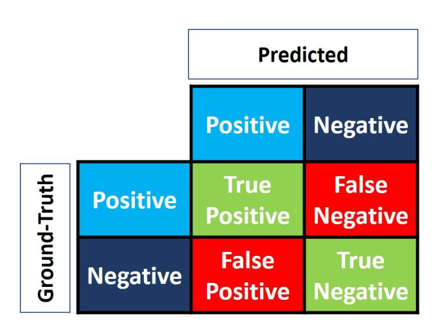
\includegraphics[]{pictures/Konfusionsmatrix_hs_analysis.png}
\subsection{Recherche und Themenfindung}

Im Rahmen der Recherche 

\subsection{Planung und Umsetzung}

Aufgrund der hohen Sicherheitsanforderungen der BWB im Rahmen der Abwasserentsorgung der kritischen Infrastruktur eines Klärwerks, bestehen grundsätzliche Vorgaben zum Arbeiten im Air Gap. Diese waren auch für dieses Projekt von Relevanz, da sämtlich Arbeitsprozesse und Lösungen entsprechend zugeschnitten werden mussten, um lokal und komplikationsarm ausführbar zu sein. Sämtliche Methoden und Lösungen sind so oder in abgewandelter Form auch für die Bachelorarbeit notwendig gewesen. 

\begin{figure}[H]
    \centering
    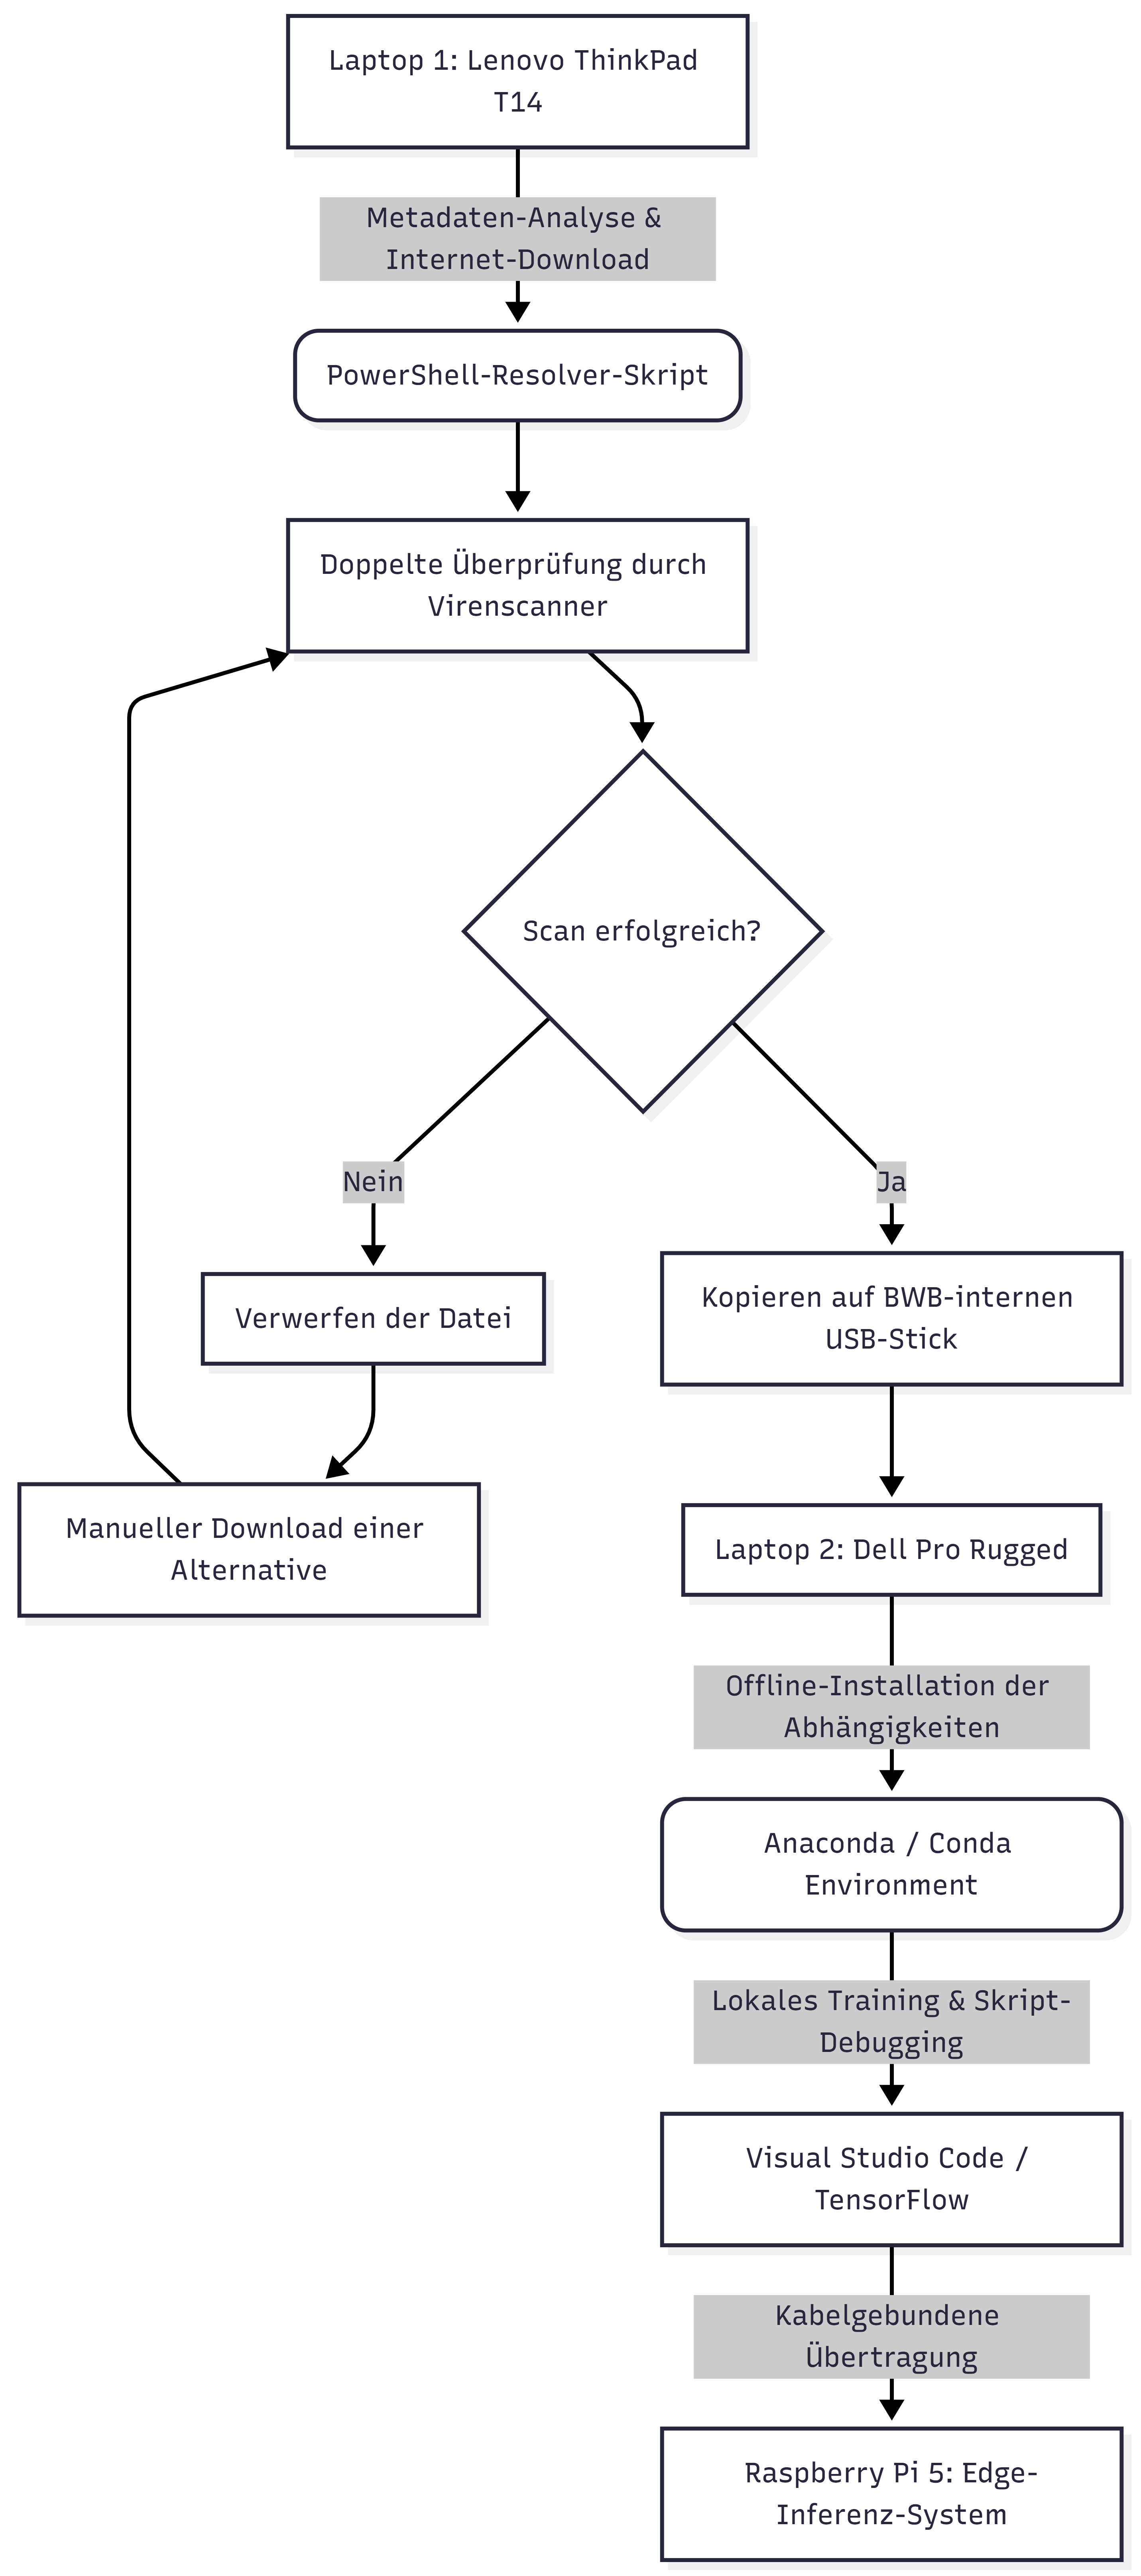
\includegraphics[width=0.5\linewidth]{pictures/Workflow.png} 
    \caption{Darstellung des Air Gaps der Arbeitsumgebung}
    \label{fig:airgap}
\end{figure}

Dieser Air Gap besteht aus zwei von den BWB zugewiesenen Laptops und einem unverschlüsselten USB-Stick. Laptop 1, ein Lenovo ThinkPad T14 liegt ohne Adminrechte und mit Windows 11 vor, um einen Internetzugang herzustellen. Auf Laptop 2 herrschen uneingeschränkte Administratorrechte, aber keine Anbindung an ein internetfähiges Netz. Dieser Laptop ist auch für die Kommunikation mit dem Raspberry PI vorgesehen. Die strikte Vorgabe besagt, dass sämtliche zu beziehenden Dateien für Laptop 2 von Laptop 1 heruntergeladen, per Virenscanner doppelt überprüft und dann auf Laptop 2 kopiert werden. Der USB-Stick ist zudem nur für die Kommunikation zwischen den firmeneigenen Endgeräten zulässig. \\ \\

Dieser Aufbau bringt vielseitige Herausforderungen mit sich, die im Alltag sonst nicht auftreten würden. So wurde auf Laptop 2 die umfassendeste Variante von Linux Mint installiert, um den Anteil an Grundfunktionen zu maximieren und den Umfang an aufwendig zu ladenden Programmen zu minimieren. Dieses Problem hätte sich grundsätzlich durch einen Endgerät mit identischem Betriebssystem lösen lassen, was hier aufgrund der Sicherheitsvorkehrungen nicht möglich war. Die Website PYPI stellt die meisten Installationsdateien mit entsprechender Versionhistorie zur Verfügung.
Mittels eines Skripts wurden die erforderlichen Abhängigkeiten (requires-dist) von Wheel-Dateien aus der METADATA ausgelesen. Hierdurch wurden Informationen wie benötigte Python- und Programmversion einer einzelnen .whl Datei oder einem Ordner ausgelesen. Mit weiteren Spezifikationen im Skript konnten die Downloads dann für die Zielplattform angepasst und iterativ gestalten werden, damit sämtliche Subdependencies aufgelöst werden konnten. Nicht zuletzt wurden herunterzulandende Inhalte mit den im Ordner vorhandenen abgeglichen um Dopplungen zu vermeiden.\\ \\



\begin{lstlisting}[caption=Powershell-Skript zum Download von Wheel Dateien]
$Path           = ".\" # Datei ODER Ordnerpfad
$DownloadDir    = ".\"
$TargetPython   = "Python_Version"
$Platform       = "Platform_Variante"
$MaxThreads     = Anzahl_Threads  # Erhoeht fuer maximale Auslastung

[Net.ServicePointManager]::SecurityProtocol = [Net.SecurityProtocolType]::Tls12
Add-Type -AssemblyName System.IO.Compression.FileSystem

if (!(Test-Path $DownloadDir)) { New-Item -ItemType Directory -Path $DownloadDir | Out-Null }
$GlobalDownloaded = [Hashtable]::Synchronized(@{})
$TotalBytesToDownload = [long]0

function Format-Size ([long]$bytes) {
    if ($bytes -gt 1GB) { return "{0:N2} GB" -f ($bytes / 1GB) }
    return "{0:N2} MB" -f ($bytes / 1MB)
}

function Get-DependenciesFromWheel {
    param($Whl)
    $deps = @()
    try {
        $zip = [System.IO.Compression.ZipFile]::OpenRead($Whl)
        $meta = $zip.Entries | Where-Object { $_.FullName -match "METADATA$" }
        if ($meta) {
            $r = New-Object System.IO.StreamReader($meta.Open())
            while ($l = $r.ReadLine()) { if ($l -match "^Requires-Dist:\s*([^;]+)") { $deps += $Matches[1].Trim() } }
            $r.Close()
        }
        $zip.Dispose()
    } catch {}
    return $deps | Select-Object -Unique
}

$RunspacePool = [RunspaceFactory]::CreateRunspacePool(1, $MaxThreads)
$RunspacePool.Open()
$Jobs = New-Object System.Collections.Generic.List[Hashtable]

function Queue-Download {
    param($RawDep)
    $name = ($RawDep -split "[\s;>=<\[,! ]")[0].ToLower().Trim()
    if ([string]::IsNullOrWhiteSpace($name) -or $GlobalDownloaded.ContainsKey($name)) { return }
    
    $PkgKey = $name.Replace(".","_")
    if (Get-ChildItem $DownloadDir | Where-Object { $_.Name.ToLower().Replace(".","_").StartsWith($PkgKey + "-") }) { 
        $GlobalDownloaded[$name] = $true; return 
    }

    $GlobalDownloaded[$name] = $true
    $targetV = $null
    if ($RawDep -match "==\s*([0-9\.]+)") { $targetV = $Matches[1].TrimEnd('.') }

    $ScriptBlock = {
        param($PkgName, $SpecificVersion, $Dir, $Target, $Platform)
        try {
            $api = Invoke-RestMethod "https://pypi.org/pypi/$PkgName/json"
            $v = if ($SpecificVersion) { $SpecificVersion } else { $api.info.version }
            $rel = $api.releases.$v
            if (!$rel) { $v = $api.info.version; $rel = $api.releases.$v }

            $valid = $rel | Where-Object { $_.filename -match "\.whl$" -and $_.filename -notmatch "macosx|win|aarch64" }
            $best = $valid | Where-Object { $_.filename -match "cp$Target" -and $_.filename -match $Platform }
            if (!$best) { $best = $valid | Where-Object { $_.filename -match "py3-none" -and $_.filename -match $Platform } }
            if (!$best) { $best = $valid | Where-Object { $_.filename -match "py3-none-any" } }
            
            if ($best) {
                $file = $best[0]
                $path = Join-Path $Dir $file.filename
                (New-Object System.Net.WebClient).DownloadFile($file.url, $path)
                return @{ Name = $PkgName; Size = $file.size; File = $file.filename; Deps = $api.info.requires_dist }
            }
        } catch { return $null }
    }

    $PS = [PowerShell]::Create().AddScript($ScriptBlock)
    .AddArgument($name).AddArgument($targetV).AddArgument($DownloadDir)
    .AddArgument($TargetPython).AddArgument($Platform)
    $PS.RunspacePool = $RunspacePool
    $Jobs.Add(@{ PS = $PS; Handle = $PS.BeginInvoke() })
}

# --- AUTOMATISCHE WEICHENSTELLUNG ---
Write-Host "`n>>> INITIALISIERE ANALYSE..." -ForegroundColor Cyan

if (Test-Path $Path -PathType Container) {
    Write-Host "[i] Modus: ORDNER-SCAN ($Path)" -ForegroundColor Gray
    Get-ChildItem $Path -Filter "*.whl" | ForEach-Object {
        $name = ($_.Name -split "-")[0].ToLower().Replace(".","_")
        $GlobalDownloaded[$name] = $true
        Get-DependenciesFromWheel $_.FullName | ForEach-Object { Queue-Download $_ }
    }
} else {
    Write-Host "[i] Modus: EINZELDATEI-SCAN ($Path)" -ForegroundColor Gray
    Get-DependenciesFromWheel $Path | ForEach-Object { Queue-Download $_ }
}

# --- REKURSIVER TURBO-LOOP ---
while ($true) {
    $running = $Jobs | Where-Object { $_.Handle.IsCompleted -eq $false }
    $finished = $Jobs | Where-Object { $_.Handle.IsCompleted -eq $true -and $_.Processed -ne $true }

    foreach ($j in $finished) {
        $res = $j.PS.EndInvoke($j.Handle)
        if ($res) {
            [System.Threading.Interlocked]::Add([ref]$TotalBytesToDownload, $res.Size) | Out-Null
            if ($res.Deps) { foreach ($nd in $res.Deps) { Queue-Download $nd } }
            Write-Host "`r  [DONE] $($res.File) ($(Format-Size $res.Size))" -ForegroundColor Green
        }
        $j.Processed = $true
    }

    $localSum = (Get-ChildItem $DownloadDir | Measure-Object -Property Length -Sum).Sum
    if (!$localSum) { $localSum = 0 }
    $perc = if ($TotalBytesToDownload -gt 0) { [Math]::Min(100, ($localSum / $TotalBytesToDownload) * 100) } else { 0 }

    Write-Host -NoNewline ("`rFortschritt: $(Format-Size $localSum)) ($ | Aktiv: $($running.Count)   ") -ForegroundColor Yellow

    if ($running.Count -eq 0 -and $finished.Count -eq 0) { 
        Start-Sleep -Seconds 1
        if (($Jobs | Where-Object { $_.Handle.IsCompleted -eq $false }).Count -eq 0) { break }
    }
    Start-Sleep -Milliseconds 400
}

$RunspacePool.Close()
Write-Host "`n`n--- FERTIG! ---" -ForegroundColor Cyan
Pause
\end{lstlisting}

\begin{figure}[H]
    \centering
    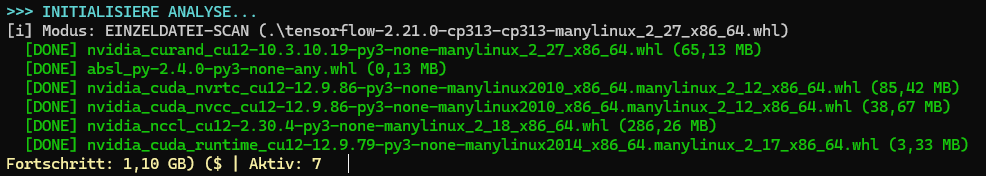
\includegraphics[width=1\linewidth]{pictures/Screenshot_Powershell_Skript.png}
    \caption{Ausführung des Powershell Skript anhand des Beispiels von Tensorflow}
    \label{fig:powershell}
\end{figure}

Wie in \ref{fig:powershell} sichtbar, durchläuft das Skript anhand einer Einzeldatei sämtlich Requires und lädt diese in der passenden Variante parallel über mehrere Threads herunter, damit bei den großen Datenmengen von insbesondere Nvidia Programmen keine überdimensionierten Laufzeiten entstehen. Außerdem wird die Größe des Zielordners und eine Übersicht die Anzahl laufender Prozesse gegeben. Falls die Anforderungen an die Dateiversionen nicht erfüllt werden können, werden stattdessen die none-any-Varianten geladen. Eine vollständige Automatisierung konnte so nicht stattfinden, weswegen einzelne Abhängigkeiten dennoch manuell geladen wurden, aber im Vergleich zur händischen Downloads stellt es trotzdem eine enorme Vereinfachung dar und kann zudem für die Installation des Raspberry PI wiederverwendet werden. \\ \\

Im Rahmen der Arbeit wurden drei unterschiedliche Environments von venv, über Miniconda zu Conda selbst hin vorgenommen. Während Miniconda bereits angenehme Arbeitsweisen ermöglichte, fiel die Wahl letztendlich auf Conda aufgrund preinstalls, da die Anzahl zu installierender Pakete hierdurch deutlich sank. Insbesondere Programme wie PIP wiesen größere Schwierigkeiten auf, da eine Offline-Installation so nicht vorgesehen ist. Der Umschwung auf das umfangreichere Anaconda ermöglichte die problemlosere Installation der weiteren requires, was auch als Option für den Raspberry Pi offen bleibt und nur an Schwierigkeiten mit der Performanz scheitern könnte. \\ \\



ARBEIT IM ENVIRONMENT --> Conda (PIP)


conda activate mud \\ 
pip install program --no-index find-links . 

\section{Produktwahl}

\begin{table}[]
    \centering
    \begin{tabular}{|l|l|}
    \hline
    \textit{\textbf{Name}}                                & \textbf{Raspberry Pi 5}                                  \\ \hline
    \textit{\textbf{Processor (CPU)}}                            & ARM Cortex-A72 quad-core processor with 1.5GHz frequency \\ \hline
    \textit{\textbf{RAM}}
    & 8GB LPDDR4                                               \\ \hline
    \textit{\textbf{Graphics (GPU)}}                             & VideoCore VI GPU, supports 4K                            \\ \hline
    \textit{\textbf{Wireless Connectivity}} & Wi-Fi 5, Bluetooth 5.0                                   \\ \hline
    \textit{\textbf{USB Ports}}                                  & 4 USB 2.0 ports, 1 USB 3.0 port                          \\ \hline
   \textit{\textbf{Ethernet}}                                   & 10/100 Mbps Ethernet                                     \\ \hline
    \textit{\textbf{Storage}}                                    & microSD (no support for internal SSD or eMMC)            \\ \hline
    \textit{\textbf{Camera Support}}                             & CSI-2 port for camera attachment                         \\ \hline
    \textit{\textbf{Power Efficiency}}                           & Average power consumption, optimized for long-term use   \\ \hline
    \textit{\textbf{GPIO Ports}}                                 & 40 programmable GPIO pins                                \\ \hline
    \textit{\textbf{Size \& Design}}                             & Standard design with size of 88x58mm                     \\ \hline
    \textit{\textbf{Price (Estimated)}}                          & Approximate price of 180€ for the advanced model             \\ \hline                              
    \end{tabular}
    \caption{Übersicht der Eigenschaften eines Raspberry Pi 5}
    \label{tab:Eigenschaftstabelle}
\end{table}

